\section{Auswertung}
\label{sec:Auswertung}

\subsection{Literaturwerte}

Die Ordnungszahlen der Stoffe, die im Versuch untersucht werden, sind in
Tabelle \ref{tab:litwerte} aufgezählt.
Die Werte für die Lichtgeschwindigkeit $c$, die Elementarladung $e$, die
Feinstrukturkonstante $\alpha$ und das Plancksche Wirkungsquantum $h$ werden aus
\cite{Codata} entnommen.

\subsection{Überprüfung der Bragg Bedingung}

In Tabelle \ref{tab:braggbed} sind die Messwerte zur Überprüfung der braggschen
Bedingung dargestellt. Diese sind in Abbildung \ref{fig:braggbed} als Graph
aufgetragen.
Das Maximum der Kurve liegt bei
\begin{align}
  \theta_\text{mess} = \SI{14.2}{\degree}.
\end{align}
Der Sollwert für das Maximum lautet
\begin{equation}
  \theta_\text{soll} = \SI{14}{\degree}.
\end{equation}

\subsection{Das Emissionsspektrum einer CU-Röntgenröhre}

In Tabelle \ref{tab:emission1}, \ref{tab:emission2}, \ref{tab:emission3} und
\ref{tab:emission4} sind die Messwerte zur Bestimmung des
Emissionsspektrum der CU-Röntgenröhre abgebildet. Der zugehörige Graph ist
ist in Abbildung \ref{fig:emission} dargestellt.
Der Grenzwinkel befindet sich bei
\begin{equation}
  \theta_\text{CU} = \SI{4.4}{\degree}.
\end{equation}
Mit der Bragg'schen Bedingung folgt dann die minimale Wellenlänge
\begin{equation}
  \lambda_\text{CU} = \SI{0.0309}{\nano\meter}
\end{equation}
bzw. die maximale Energie, bei der die Elektronen vollständig abgebremst werden,
\begin{equation}
  E_\text{CU} = \SI{40.1208}{\kilo\electronvolt}.
\end{equation}
In den Abbildungen \ref{fig:emissionkalpha} und \ref{fig:emissionkbeta} sind
jeweils die Messwerte an der $K_\alpha$- und $K_\beta$- Linie des
Emissionsspektrums abgebildet. Diese werden jeweils durch ein Polynom zweiten
Grades angenähert.
Die Hochpunkte der Parabeln sind bei
\begin{align}
  \theta_\alpha = & \SI{22.1098}{\degree} \\
  \theta_\beta = & \SI{19.8107}{\degree}.
\end{align}
Daraus folgen die Halbwerte
\begin{align}
  \theta_{\alpha 1} = & \SI{21.8759}{\degree} \\
  \theta_{\alpha 2} = & \SI{22.3438}{\degree} \\
  \theta_{\beta 1} = & \SI{19.5047}{\degree} \\
  \theta_{\beta 2} = & \SI{20.1167}{\degree}.
\end{align}
Durch bilden der Differenzen ergeben sich die Halbwertsbreiten der
$K_\alpha$- und $K_\beta$- Linie
\begin{align}
  \increment \theta_\alpha = & \SI{0.4679}{\degree} \\
  \increment \theta_\beta = & \SI{0.6120}{\degree}.
\end{align}
Die Energieauflösung ergibt sich aus dem Mittelwert der Energieauflösungen
der $K_\alpha$- und $K_\beta$- Linie
\begin{equation}
  \increment E = \frac{1}{2}(\increment E_\alpha + \increment E_\beta) \pm
  \sqrt{(\increment E_\alpha - \bar{E})^2 + (\increment E_\beta - \bar{E})^2}
  = \SI{172(138)}{\electronvolt}.
\end{equation}
Es folgen mit \eqref{eqn:sigmaK}
die Abschirmkonstanten an der K-Kante von Kupfer
\begin{align}
  \sigma_\text{1,CU,mess} & = z_\text{CU} - \sqrt{\frac{E_{K_\beta}}{R_\infty}} & = 3.16 \\
  \sigma_\text{2,CU,mess} & = z_\text{CU} - 2\sqrt{\frac{(E_{K_\beta}-E_{K\alpha})}{R_\infty}} & = 12.69.
\end{align}

\subsection{Absorptionsspektren verschiedener Stoffe}

\subsubsection{Germanium}

Die Messwerte der Germaniumprobe sind in Tabelle \ref{tab:germanium1} und
\ref{tab:germanium2} abgebildet
und als Graph in Abbildung \ref{fig:germanium} aufgetragen.
Die gemessene K-Kante befindet sich bei
\begin{equation}
  \theta_\text{Ge} = \SI{16.2}{\degree}.
\end{equation}
Mit der Bragg'schen Bedingung \eqref{eqn:braggbed} folgt dann für die
Wellenlänge
\begin{equation}
  \lambda_\text{Ge} = \SI{0.1124}{\nano\meter}.
\end{equation}
Mit der Formel
\begin{equation}
  E = \frac{c h}{\lambda}
  \label{eqn:energielambda}
\end{equation}
folgt der Energiewert an der K-Kante für Germanium
\begin{equation}
  E_\text{Ge,mess} = \SI{11.0328}{\kilo\electronvolt}.
\end{equation}
Mit \eqref{eqn:sigmaK} folgt die Abschirmzahl an der K-Kante von Germanium
\begin{align}
  \sigma_\text{K,Ge,mess} = 3.7639.
\end{align}

\subsubsection{Brom}

Die Messwerte der Bromprobe sind in Tabelle \ref{tab:brom1} und \ref{tab:brom2}
dargestellt und als
Graph in der Abbildung \ref{fig:brom} aufgetragen.
Die gemessene K-Kante befindet sich bei
\begin{equation}
  \theta_\text{Br} = 12.7 .
\end{equation}
Für die Wellenlänge folgt mit \eqref{eqn:braggbed}
\begin{equation}
  \lambda_\text{Br} = \SI{0.0886}{\nano\meter}.
\end{equation}
Daraus ergibt sich mit Hilfe der Formel \eqref{eqn:energielambda}
der Wert am Energieübergang
\begin{equation}
  E_\text{Br,mess} = \SI{14.0008}{\kilo\electronvolt}.
\end{equation}
Mit \eqref{eqn:sigmaK} folgt die Abschirmkonstante an der K-Kante von Brom
\begin{align}
  \sigma_\text{K,Br,mess} = 3.2274.
\end{align}

\subsubsection{Zirkonium}

Die Messwerte für Zirkonium sind in den Tabellen \ref{tab:zirkonium1} und
\ref{tab:zirkonium2} dargestellt und
in Abbildung \ref{fig:zirkonium} als Graph aufgetragen.
Die K-Kante wird bei
\begin{equation}
  \theta_\text{Zr} = \SI{9.4}{\degree}
\end{equation}
gemessen.
Daraus folgt mit \eqref{eqn:braggbed} die Wellenlänge
\begin{equation}
  \lambda_\text{Zr} = \SI{0.0658}{\nano\meter}.
\end{equation}
Mit \eqref{eqn:energielambda} folgt der Energiewert von Zirkonium an der
K-Kante
\begin{align}
  E_\text{Zr,mess} = \SI{18.8459}{\kilo\electronvolt}.
\end{align}
Die Abschirmkostante ergibt sich mit der Formel \eqref{eqn:sigmaK}
\begin{align}
  \sigma_\text{K,Zr,mess} = 3.2352.
\end{align}

\subsubsection{Bismuth}

In Tabelle \ref{tab:bismuth1} und \ref{tab:bismuth2} sind die Messwerte der
Bismuthprobe abgebildet.
Diese sind in Abbildung \ref{fig:bismuth} als Graph aufgetragen.
Die Messung ergibt einen Winkel von
\begin{align}
  \theta_\text{Bi,LII} = \SI{10.7}{\degree}
\end{align}
an der LII-Kante und einen Winkel von
\begin{align}
  \theta_\text{Bi,LIII} = \SI{12.8}{\degree}
\end{align}
an der LIII-Kante.
Daraus ergeben sich mit \eqref{eqn:braggbed} die Wellenlängen
\begin{align}
  \lambda_\text{Bi,LII} = \SI{0.0748}{\nano\meter}
\end{align}
und
\begin{align}
  \lambda_\text{Bi,LIII} = \SI{0.0892}{\nano\meter}.
\end{align}
Mit \eqref{eqn:energielambda} folgt der Energiedifferenzwert der L-Kanten von
Bismuth
\begin{align}
  E_\text{Bi,mess} = \SI{2.7850}{\kilo\electronvolt}.
\end{align}
Daraus ergibt sich mit \eqref{eqn:sigmal} die Abschirmkonstante der L-Schale
von Bismuth
\begin{align}
  \sigma_\text{L,Bi,mess} = 0.7988.
\end{align}

\subsection{Das Moseleysche Gesetz}

In Abbildung \ref{fig:moseley} sind die berechneten Absorptionsenergien und die
Kernladungszahlen für Germanium, Brom und Zirkonium in einem
$\sqrt{E_k}-Z$-Diagramm dargestellt. Durch die Werte wird eine Ausgleichsgerade
gelegt, die ausgegebene Steigung beträgt
\begin{align}
  m = \num{0.25(1)}.
\end{align}
Daraus ergibt sich die Rydbergkonstante
\begin{align}
  R_\text{\infty, mess} = \SI{22(2)}{\per\meter}.
\end{align}

\begin{figure}
  \centering
  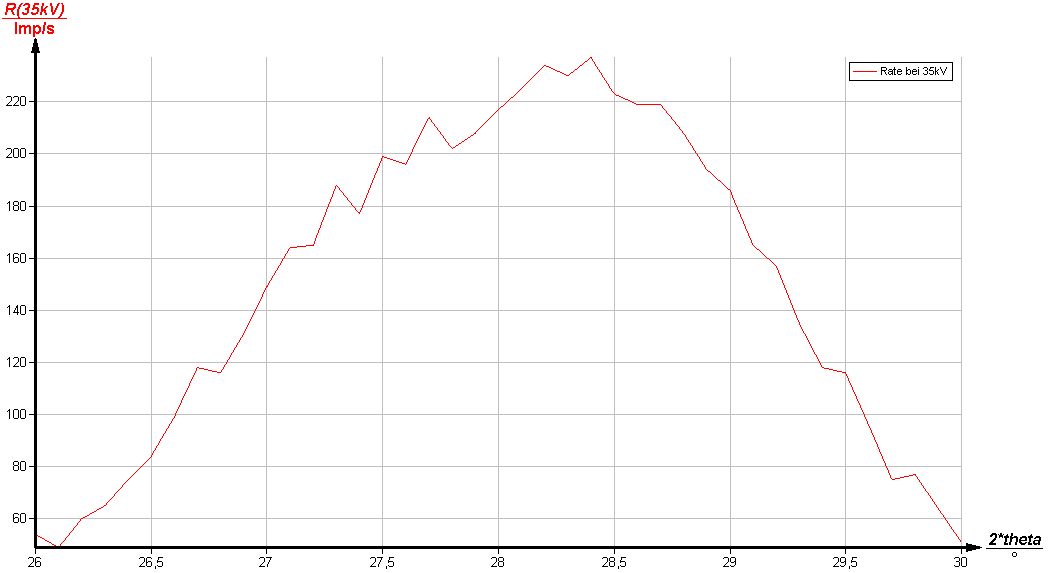
\includegraphics[height=9cm]{Daten/braggbedingung.png}
  \caption{Graph zur Überprüfung der Bragg Bedingung. Es sind die Impulse pro
  Sekunde gegen den Winkel aufgetragen.}
  \label{fig:braggbed}
\end{figure}

\begin{figure}
  \centering
  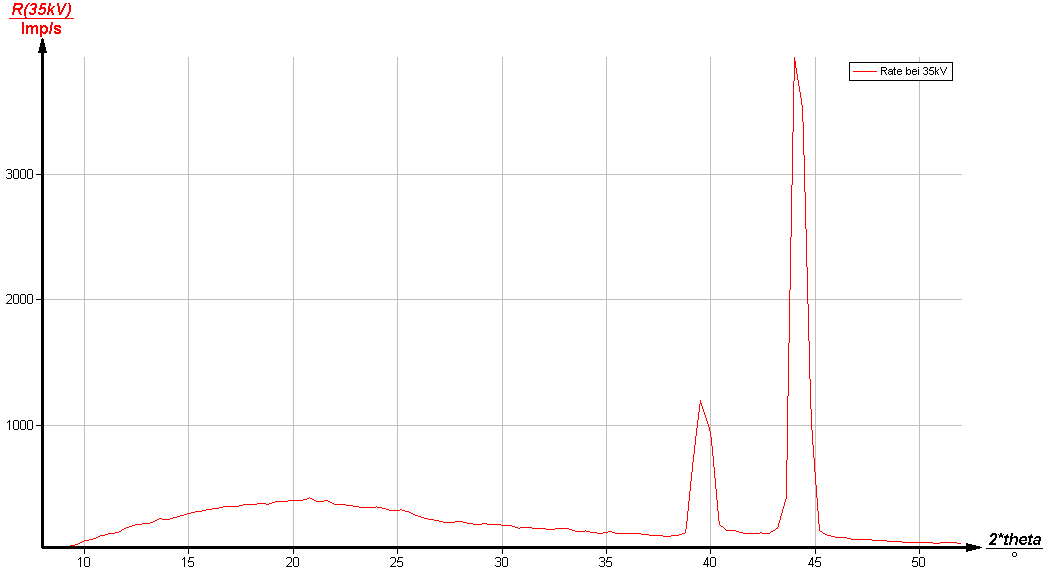
\includegraphics[height=8cm]{Daten/emissionsspektrum.png}
  \caption{Graph des Emissionsspektrums der CU-Röntgenröhre. Es sind die
  Impulse pro Sekunde gegen den Winkel aufgetragen.}
  \label{fig:emission}
\end{figure}

\begin{figure}
  \centering
  \includegraphics[height=8cm]{build/emissionsspektrumKbetha.pdf}
  \caption{Messwerte der $K_\alpha$-Linie des Emissionsspektrums der
  CU-Röntgenröhre und Ausgleichspolynom. Es sind die
  Impulse pro Sekunde gegen den Winkel aufgetragen.}
  \label{fig:emissionkalpha}
\end{figure}

\begin{figure}
  \centering
  \includegraphics[height=8cm]{build/emissionsspektrumKalpha.pdf}
  \caption{Messwerte der $K_\beta$-Linie des Emissionsspektrums der
  CU-Röntgenröhre und Ausgleichspolynom. Es sind die Impulse pro Sekunde
  gegen den Winkel aufgetragen.}
  \label{fig:emissionkbeta}
\end{figure}

\begin{figure}
  \centering
  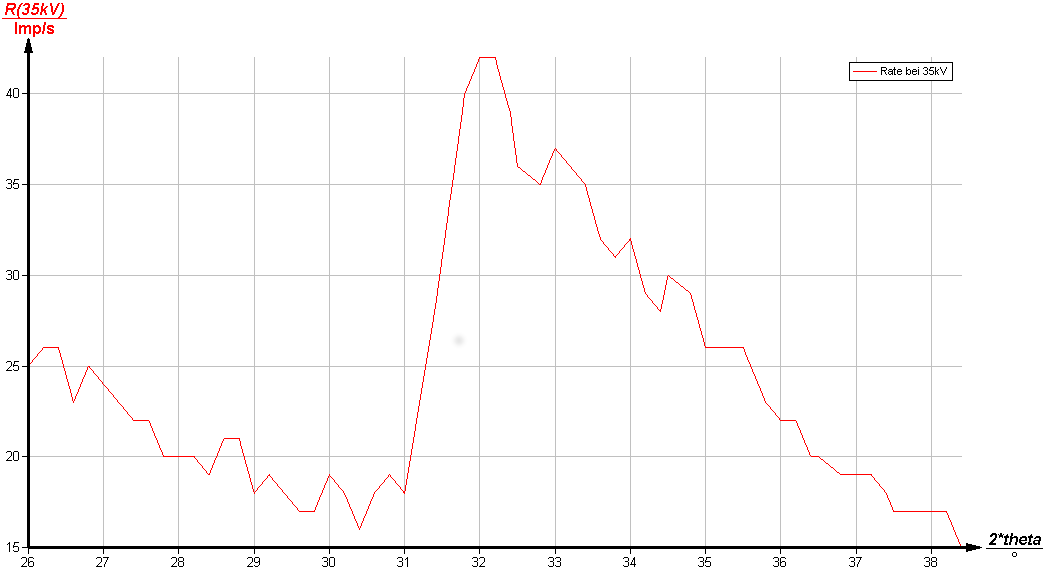
\includegraphics[height=8cm]{Daten/germanium.png}
  \caption{Graph der Messwerte des Absorptionsspektrums der Germaniumprobe. Es
  sind die Impulse pro Sekunde gegen den Winkel aufgetragen.}
  \label{fig:germanium}
\end{figure}

\begin{figure}
  \centering
  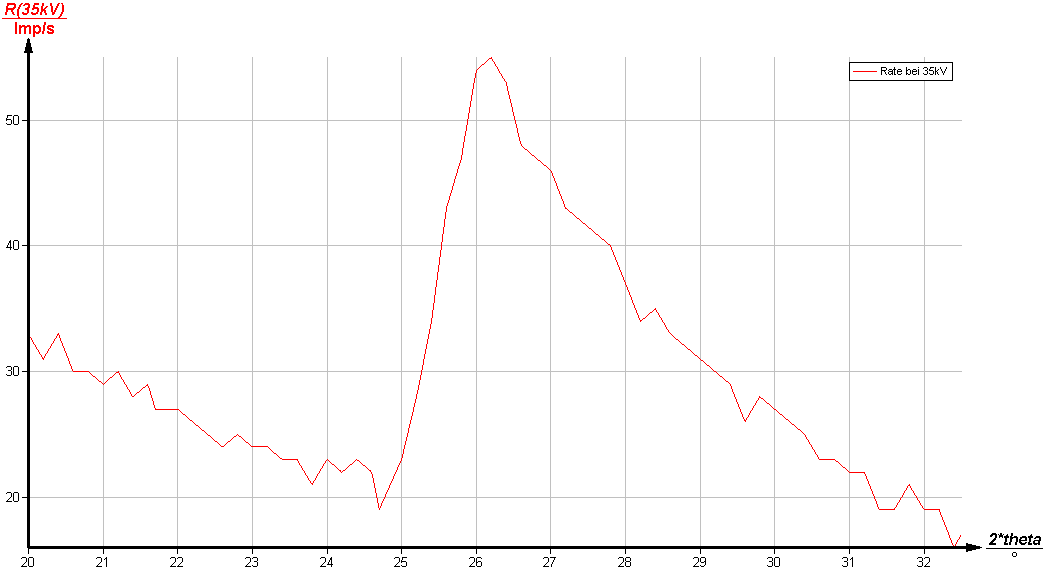
\includegraphics[height=8cm]{Daten/brom.png}
  \caption{Graph der Messwerte des Absorptionsspektrums der Bromprobe. Es
  sind die Impulse pro Sekunde gegen den Winkel aufgetragen.}
  \label{fig:brom}
\end{figure}

\begin{figure}
  \centering
  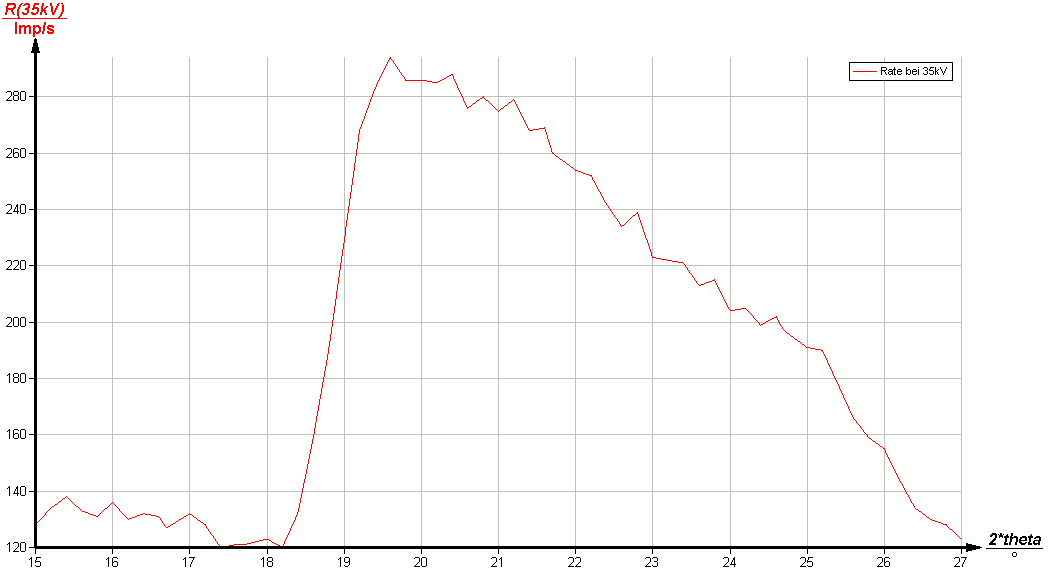
\includegraphics[height=8cm]{Daten/zirkonium.png}
  \caption{Graph der Messwerte des Absorptionsspektrums der Zirkoniumprobe. Es
  sind die Impulse pro Sekunde gegen den Winkel aufgetragen.}
  \label{fig:zirkonium}
\end{figure}

\begin{figure}
  \centering
  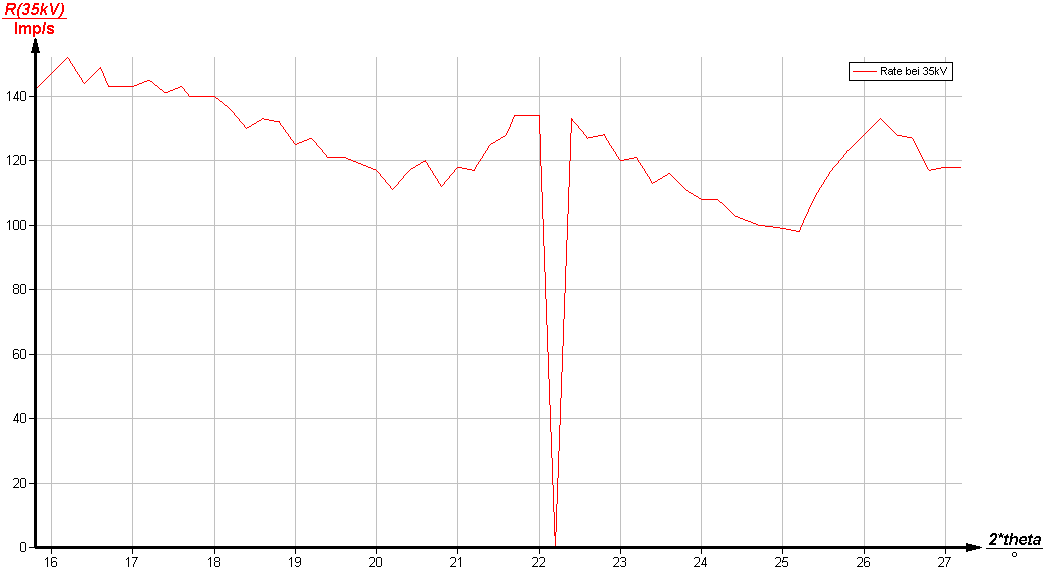
\includegraphics[height=8cm]{Daten/bismuth.png}
  \caption{Graph der Messwerte des Absorptionsspektrums der Bismuthprobe. Es
  sind die Impulse pro Sekunde gegen den Winkel aufgetragen.}
  \label{fig:bismuth}
\end{figure}

\begin{figure}
  \centering
  \includegraphics[height=8cm]{build/Moseley.pdf}
  \caption{Graph zur Bestimmung der Rydbergkonstante. Es ist $\sqrt{E_k}$ gegen
  Z aufgetragen.}
  \label{fig:moseley}
\end{figure}
